%%%%%%%%%%%%%%%%%%%%%%%%%%%%%%%%%%%%%%
%
% This is how you write code:
%
% \begin{minted}{matlab}
% foo = [2 1 0;1 4 3;2 4.5 6];
% \end{minted}
%

% This is how you import code:
% 
% \inputminted[linenos]{matlab}{foo_bar.m}
%
 
% Most figures are imported this way:
%
% \begin{figure}
% \includegraphics[width=\textwidth]{foo_figure}
% \caption{This is a caption}
% \end{figure}

% This is a matrix:
%
% \begin{equation}
% H =
%  \left[
%  \begin{matrix}
%    1 & 2 &  3 &  4 \\ 
%    5 & 6 &  7 &  8 \\ 
%    0 & 9 & 10 & 11 \\ 
%    0 & 0 & 12 &  0
%  \end{matrix} 
% \right]
%\end{equation}
%
%%%%%%%%%%%%%%%%%%%%%%%%%%%%%%%%%%%%%%


\documentclass[00-main.tex]{subfiles}
\begin{document}




\section*{Problem One}

\subsection*{a.}

\begin{figure}
  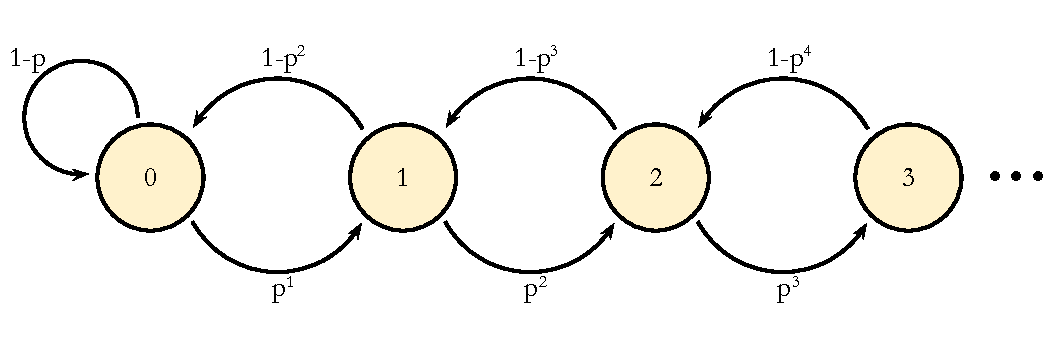
\includegraphics[width=\textwidth]{markov-chain.pdf}
  \caption{The Markov chain $P_{ij}$ illustrated as a digraph.}
  \label{markov}
\end{figure}

The Markov chain $P_{ij}$ in \ref{markov} describes a random walk. Starting in any state, you can reach any other state - i.e. all states communicate. 
Thus, $P_{ij}$ is \textbf{strongly connected}, has \textbf{one equivalence class} and is \textbf{irreducible}. 
Let $X_n$ and $X_{n+s}$ be two states such that there are $s-1$ intermediate states between them. 
To get from state $i$ to $j=i+s$ you have to visit all ($s-1$) intermediate states at least once\footnote{Equivalently, $s$ is the minimum number of steps you must preform to make the transition from state $i$ to $i+s$}. 
Another trait of $P_{ij}$ is that the probability of moving from state $i$ to $j=i+1$ diminishes exponentially with growing $i$. 
Starting in state $i$, it is always possible to return to state $i$ in a finite number of steps.
State $i$ is then said to be positive recurrent, and since positive recurrence is a class property, the whole chain is \textbf{positive recurrent}.

Starting in state $i$, let $n$ be the number that allows you to end up in state $i$ after $n$ transitions with the probability $P^{n}_{ii} > 0$. 
Let $N_i$ be the set of all such numbers for our chain. 
The greatest common divisor of the elements in $N_i$ is called the period $d$ of  state $i$.
Since $P^{n}_{00} > 0$ for any $n$, $N_i = 0, 1, 2, ...$ and so $P_{00}$ has a period of $d=1$. Since periodicity is a class property, the chain as a whole has period of one. 
A Markov chain with $d=1$ is called \textbf{aperiodic}.









\end{document}